\section{Өгөгдлийн сангийн диаграмм}
\begin{figure}[ht]
  \centering
  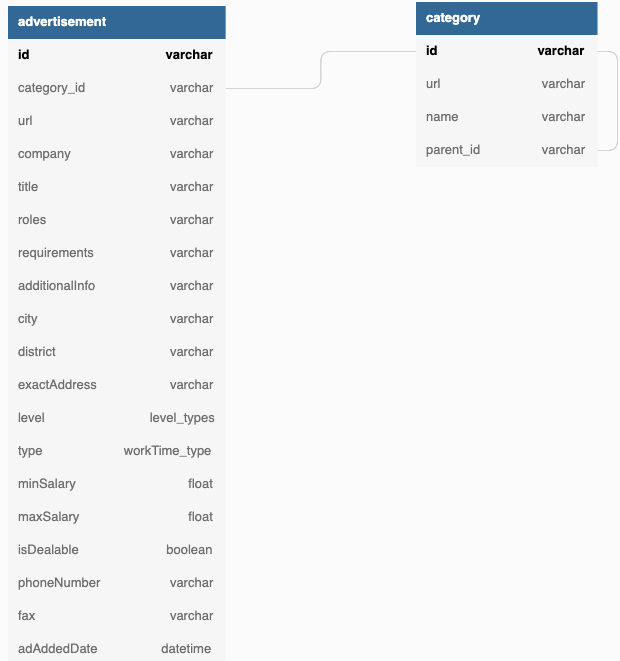
\includegraphics[width = \textwidth-2cm]{images/dbDiagram.png}
  \caption{Өгөгдлийн сангийн диаграмм}\label{fig:dbDiagram}
\end{figure}
\newpage

\section{Өгөгдлийн элемент}
Чатбот системийн өгөгдлийн сангийн диаграммд харуулсан хүснэгтүүдэд агуулагдах мэдээлэл болон үүргийн талаар дэлгэрэнгүй тайлбарласан болно. 
\subsection{advertisement - Ажлын байрны зар}
Ажлын байрны зар нь ямар категори буюу ангилалд, ямар холбоо барих хаягийн хамтаар хадгалагдаж буй мэдээлэл болон бусад дэлгэрэнгүй мэдээллийг харуулсан байна. 
\begin{table}[ht]
  \begin{tabular}{|l|l|c|c|c|l|}
  \hline
  \multicolumn{1}{|c|}{\textbf{№}} & \multicolumn{1}{c|}{\textbf{Баганын нэр}} & \textbf{\begin{tabular}[c]{@{}c@{}}Түлхүүр \\ өгөгдөл\end{tabular}} & \textbf{\begin{tabular}[c]{@{}c@{}}Өгөгдлийн\\ төрөл\end{tabular}} & \textbf{\begin{tabular}[c]{@{}c@{}}Хоосон\\ утга\end{tabular}} & \multicolumn{1}{c|}{\textbf{Тайлбар}}                                                  \\ \hline
  1                                & \textbf{\_id}                             & PK                                                                  & varchar                                                            & not null                                                       & \begin{tabular}[c]{@{}l@{}}Ажлын байрны зарын дахин\\ давтагдашгүй дугаар\end{tabular} \\ \hline
  2                                & category\_id                              & FK                                                                  & varchar                                                            & not null                                                       & \begin{tabular}[c]{@{}l@{}}Ажлын байрны зард хамаарах\\ ангилалын дугаар\end{tabular}  \\ \hline
  3                                & url                                       &                                                                     & varchar                                                            & not null                                                       & Ажлын байрны зарын хаяг                                                                \\ \hline
  4                                & company                                   &                                                                     & varchar                                                            & not null                                                       & Ажил олгогч компани / хувь хүн                                                         \\ \hline
  5                                & title                                     &                                                                     & varchar                                                            & not null                                                       & Ажлын зарын гарчиг                                                                     \\ \hline
  6                                & roles                                     &                                                                     & varchar                                                            & null                                                           & Гүйцэтгэхүндсэн үүрэг                                                                  \\ \hline
  7                                & requirements                              &                                                                     & varchar                                                            & null                                                           & \begin{tabular}[c]{@{}l@{}}Ажлын байранд тавигдах\\ шаардлага\end{tabular}             \\ \hline
  8                                & additionalInfo                            &                                                                     & varchar                                                            & null                                                           & Нэмэлт мэдээлэл                                                                        \\ \hline
  9                                & city                                      &                                                                     & varchar                                                            & null                                                           & Ажлын байрны харъяа хот                                                                \\ \hline
  10                               & district                                  &                                                                     & varchar                                                            & null                                                           & Ажлын байрны харъяа дүүрэг                                                             \\ \hline
  11                               & exactAddress                              &                                                                     & varchar                                                            & null                                                           & Ажлын байрны бүтэн хаяг                                                                \\ \hline
  12                               & level                                     &                                                                     & level\_types                                                       & null                                                           & Ажлын түвшин                                                                           \\ \hline
  13                               & type                                      &                                                                     & workTime\_type                                                     & null                                                           & Ажиллах цагийн төрөл                                                                   \\ \hline
  \end{tabular}
  \end{table}
\begin{table}[ht]
  \caption{advertisement хүснэгт}\label{table:advertisement}
    \begin{tabular}{|l|l|c|c|c|l|}
    \hline
    \multicolumn{1}{|c|}{\textbf{№}} & \multicolumn{1}{c|}{\textbf{Баганын нэр}} & \textbf{\begin{tabular}[c]{@{}c@{}}Түлхүүр \\ өгөгдөл\end{tabular}} & \textbf{\begin{tabular}[c]{@{}c@{}}Өгөгдлийн\\ төрөл\end{tabular}} & \textbf{\begin{tabular}[c]{@{}c@{}}Хоосон\\ утга\end{tabular}} & \multicolumn{1}{c|}{\textbf{Тайлбар}} \\ \hline
    14                               & minSalary                                 &                                                                     & float                                                              & null                                                           & Доод цалин                            \\ \hline
    15                               & maxSalary                                 &                                                                     & float                                                              & null                                                           & Дээд цалин                            \\ \hline
    16                               & isDealable                                &                                                                     & boolean                                                            & null                                                           & Цалин тохиролцох эсэх                 \\ \hline
    17                               & phoneNumber                               &                                                                     & varchar                                                            & null                                                           & Холбоо барих утасны дугаар            \\ \hline
    18                               & fax                                       &                                                                     & varchar                                                            & null                                                           & Холбоо барих факсын дугаар            \\ \hline
    19                               & publishedDate                             &                                                                     & datetime                                                           & not null                                                       & Зар нийтэлсэн огноо                   \\ \hline
    \end{tabular}
  \end{table}
Энд \textit{level} буюу ажлын түвшин, \textit{type} буюу ажлын цагийн өгөгдлийн төрлийг тодорхойлохдоо дараах байдлаар зааж өгсөн.
\\\textbf{Enum level\_types} буюу ажлын түвшний шаардлага нь дараах үндсэн 4 өгөгдлийн төрлөөс хамаарна:
\begin{itemize}
  \item student - Оюутан / дадлагажигч
  \item professional - Мэргэжлийн
  \item occupasionDoesntRequire - Мэргэжил шаардахгүй
  \item intermediateManagemet - Дунд шатны удирдлага
  \item topLevelManagemet - Дээд шатны удирдлага
\end{itemize}
\textbf{workTime\_type} буюу ажиллах цагийн нөхцөл нь дараах үндсэн 4 өгөгдлийн төрлөөс хамаарна:
\begin{itemize}
  \item shift - Ээлжийн
  \item fullTime - Бүтэн цагийн
  \item halfTime - Хагас цагийн
  \item contract - Гэрээт / зөвлөх
  \item seasonal - Улирлаар
\end{itemize}

\subsection{category - Ангилал}
Ажлын байрны зарын бүх ангиллуудын хаяг болон нэрийн мэдээллийг хадгалах хүснэгт юм. Ангиллууд нь дэд ангилал байж болох учир түүнийг эцэг ангиллын дугаарыг хадгалах байдлаар зохиомжлов. 
\begin{table}[ht]
  \caption{category хүснэгт}\label{table:category}
  \begin{tabular}{|l|l|c|l|c|l|}
  \hline
  \multicolumn{1}{|c|}{\textbf{№}} & \multicolumn{1}{c|}{\textbf{Баганын нэр}} & \textbf{\begin{tabular}[c]{@{}c@{}}Түлхүүр\\ өгөгдөл\end{tabular}} & \multicolumn{1}{c|}{\textbf{\begin{tabular}[c]{@{}c@{}}Өгөгдлийн\\ төрөл\end{tabular}}} & \textbf{\begin{tabular}[c]{@{}c@{}}Хоосон\\ Утга\end{tabular}} & \multicolumn{1}{c|}{\textbf{Тайлбар}}                                   \\ \hline
  1                                & \textbf{id}                               & PK                                                                 & varchar                                                                                 & not null                                                       & \begin{tabular}[c]{@{}l@{}}Ажлын байрны зарын\\ ангиллын дугаар\end{tabular} \\ \hline
  2                                & url                                       &                                                                    & varchar                                                                                 & not null                                                       & Ангиллын хаяг                                                          \\ \hline
  3                                & name                                      &                                                                    & varchar                                                                                 & not null                                                        & Ангиллын нэр                                                           \\ \hline
  4                                & parent\_id                                & FK                                                                 & varchar                                                                                 & null                                                           & Эцэг ангиллын дугаар                                                   \\ \hline
  \end{tabular}
\end{table}

\section{Өгөгдлийн сангийн холбоосын тайлбар}
\begin{itemize}
  \item Нэг ангилал буюу категорид олон ажлын байрны зар байж болно.
  \item Нэг ангилал буюу категорид олон категори байж болно. 
  \item Нэг ажлын байрны зард нэг категори байна.
\end{itemize}